\section{Implementazione Seriale}
\label{sec:implementazione-seriale}

L'implementazione sequenziale è il riferimento dell'intero lavoro: produce la
matrice degli escape time con cui ogni variante parallela deve coincidere e
fornisce il tempo $T_1$ rispetto al quale sono definiti speedup ed efficienza.
Questa sezione applica gli strumenti introdotti nella
sezione~\ref{sec:metriche-seriale} e ne ricava i valori numerici.

Si discute anzitutto l'effetto dei due parametri di campionamento, la
risoluzione $W \times H$ e la soglia iterativa $N_{\max}$, sul carico
computazionale e sull'accuratezza dell'immagine; si riporta poi il kernel di
escape time; si presentano infine le misure che fissano $\mathcal{W}$, $\tau$,
$\lambda$, $\mathrm{CoV}$ e il checksum della configurazione di riferimento,
verificando sui dati il modello $T_1 = \tau\,\mathcal{W}$. Il profilo di carico
e la matrice degli escape time così misurati sono l'unico ingresso delle
previsioni sulle versioni parallele, presentate insieme ai rispettivi paradigmi.
Tutte le misure sono prese sul kernel \emph{bare}, con pre-screening e simmetria
disattivati per le ragioni esposte nella sezione~\ref{sec:ottimizzazioni}.

\subsection{Impatto della risoluzione e della soglia iterativa}
\label{sec:parametri}
Il carico computazionale del codice seriale dipende da due parametri: la
risoluzione $W \times H$ fissa il numero di pixel da calcolare, la soglia
$N_{\max}$ limita il numero di iterazioni per pixel. Il lavoro totale
$\mathcal{W}$ è il prodotto dei due effetti, cioè il numero di pixel per il
numero medio di iterazioni per pixel.

\begin{itemize}
  \item \textbf{Risoluzione $W \times H$.} La griglia determina il numero di task
  indipendenti: raddoppiando sia $W$ che $H$, i pixel, e con essi il lavoro,
  quadruplicano. È l'asse che definisce la dimensione del problema. Una
  risoluzione maggiore campiona inoltre il frattale più finemente, esponendo la
  struttura del bordo.

  \item \textbf{Soglia iterativa $N_{\max}$.} Il parametro non altera il numero
  di pixel, ma limita quanto a fondo si segue ciascuna orbita. I punti esterni a
  fuga rapida escono ben prima della soglia e ne sono insensibili; i punti
  interni la raggiungono sempre, e il loro costo cresce linearmente con
  $N_{\max}$. Una soglia troppo bassa classifica come interni i punti esterni a
  fuga lenta, che nell'immagine risultano neri pur non appartenendo all'insieme;
  aumentarla corregge l'errore a un costo concentrato sui punti interni e di
  bordo.
\end{itemize}

I dati della sezione~\ref{serial_results} mostrano che la correzione riguarda
una frangia sottile lungo il contorno, di area fissa e pari a circa lo
$0{,}114\%$ della finestra, e che lo sbilanciamento del carico dipende dalla
geometria dell'insieme molto più che dalla soglia.

\subsection{Frammenti di codice rilevanti}
\label{sec:seriale-codice}
Il codice sorgente completo di tutte le implementazioni, insieme ai job script
e agli script di analisi, è disponibile nel repository del
progetto\footnote{\repolink}; il codice e i dati citati in questo elaborato corrispondono alla versione
\repoversion. Il repository separa il kernel di
calcolo, unico file riscritto per ciascun paradigma, dal codice condiviso di
driver, I/O e metriche, che resta identico in tutte le implementazioni; nel
testo si riportano soltanto i frammenti necessari alla discussione, con un
rinvio al file completo.

Di seguito si riporta il kernel seriale, tratto da
\repofile{mandelbrot/src/mandelbrot.cpp}.
\begin{lstlisting}[language=C++, caption={Kernel seriale di escape time, senza le righe relative alla simmetria.}]
MandelbrotImage compute_mandelbrot(const Viewport& view, int width, int height,
                                   int max_iter) {
    MandelbrotImage img;
    img.width = width;
    img.height = height;
    img.max_iter = max_iter;
    img.data.resize(static_cast<std::size_t>(width) * height);

    const double dx = (view.x_max - view.x_min) / width;
    const double dy = (view.y_max - view.y_min) / height;

    for (int row = 0; row < height; ++row) {
        const double c_imag = view.y_max - (row + 0.5) * dy;
        for (int col = 0; col < width; ++col) {
            const double c_real = view.x_min + (col + 0.5) * dx;
            img.data[static_cast<std::size_t>(row) * width + col] =
                escape_time(c_real, c_imag, max_iter);
        }
    }
    return img;
}

int escape_time(double c_real, double c_imag, int max_iter) {
    double z_real = 0.0;
    double z_imag = 0.0;
    double z_real_sq = 0.0;
    double z_imag_sq = 0.0;

    int iter = 0;
    while (iter < max_iter && z_real_sq + z_imag_sq <= ESCAPE_RADIUS_SQ) {
        z_imag = 2.0 * z_real * z_imag + c_imag;
        z_real = z_real_sq - z_imag_sq + c_real;
        z_real_sq = z_real * z_real;
        z_imag_sq = z_imag * z_imag;
        ++iter;
    }
    return iter;
}
\end{lstlisting}

Il frammento traduce direttamente lo pseudocodice della
sezione~\ref{pseudo}, e tre suoi dettagli condizionano il resto del lavoro. Il
ciclo esterno scorre le righe e quello interno le colonne, e la matrice è
scritta in ordine row-major: è la riga l'unità che OpenMP e MPI distribuiscono
fra le unità di calcolo. Ogni pixel è campionato nel proprio centro, il termine
$+\,0{,}5$, con la stessa espressione che tutte le implementazioni parallele
riproducono.

Nella ricorrenza, infine, la parte immaginaria è aggiornata prima di quella
reale, e i quadrati sono ricalcolati solo dopo entrambe: ogni aggiornamento usa
così i valori dell'iterazione precedente. L'ordine è necessario alla
correttezza, e tenerlo identico in ogni implementazione è parte del contratto di
riproducibilità (sezione~\ref{sec:artefatto}).

\subsection{Risultati e discussione}
\label{serial_results}
I risultati di questa sezione costituiscono la baseline per l'analisi dei codici
paralleli. Le misure provengono dal job batch $31391$, eseguito sul nodo
\texttt{gnode01}, a cui si aggiungono le due risoluzioni maggiori, $2048^2$ e
$4096^2$, misurate dal seriale del job $34424$ sullo stesso nodo. Ogni
configurazione è ripetuta $R = 3$ volte e se ne riporta il minimo
secondo~\eqref{eq:T1}.

\vspace{2,5mm}

\begin{table}[H]
    \centering
    \resizebox{\textwidth}{!}{%
    \begin{tabular}{cccccccc}
        \hline
        \textbf{$N_{\max}$} & \textbf{$T_1$} [s] & \textbf{$\mathcal{W}$} & \textbf{$\tau$} [ns] & \textbf{pixel interni (frazione)}\footnotemark & \textbf{$\lambda$} & \textbf{CoV} & \textbf{checksum}\footnotemark\\ \hline
        500 & 0{,}36703 & 132\,831\,952 & 2{,}763 & 254\,074 (24{,}230\%) & 2{,}7236 & 0{,}9485 & \texttt{25a3589a73736fcb} \\
        1000 & 0{,}72233 & 259\,655\,490 & 2{,}782 & 253\,372 (24{,}163\%) & 2{,}7638 & 0{,}9680 & \texttt{7fba3b93a2fa2397} \\
        5000 & 3{,}55817 & 1\,271\,586\,860 & 2{,}798 & 252\,858 (24{,}114\%) & 2{,}8031 & 0{,}9854 & \texttt{f25625fed7ed57c7} \\
    \end{tabular}%
    }
    \caption{Baseline seriale al variare di $N_{\max}$, a risoluzione $1024 \times 1024$ (job $31391$).}
    \label{tab:serial_var_Nmax}
\end{table}
\footnotetext{Il conteggio dei pixel interni --- come le immagini discusse
nella sezione~\ref{serial_results} e i dati della
Tabella~\ref{tab:serial_frangia} --- proviene da un'esecuzione locale della
stessa configurazione, non dal job del cluster. Le due esecuzioni sono però
sovrapponibili: producono la medesima matrice degli escape time, come attesta
l'identità dei checksum e di $\mathcal{W}$ riportati in questa stessa riga.
A cambiare fra le due è soltanto il tempo di calcolo, l'unica grandezza
dipendente dalla macchina.}
\footnotetext{I checksum sono riportati in esadecimale, come li stampa l'eseguibile; il
dataset li registra in forma decimale.  Si osservi che sono quasi tutti
distinti, coerentemente con quanto anticipato: il checksum identifica una
configurazione, e l'invarianza che verifica è quella \emph{fra le quattro
implementazioni a parità di input}, non fra input diversi.}
\setcounter{checksumfootnote}{\value{footnote}}

\vspace{2,5mm}

\begin{table}[H]
    \centering
    \begin{tabular}{ccccccc}
        \hline
        \textbf{Risoluzione} & \textbf{$T_1$} [s] & \textbf{$\mathcal{W}$} & \textbf{$\tau$} [ns] & \textbf{$\lambda$} & \textbf{CoV} & \textbf{checksum}\footnotemark[\value{checksumfootnote}]\\ \hline
        $512 \times 512$   & 0{,}18084  & 64\,917\,922      & 2{,}786 & 2{,}7646 & 0{,}9679 & \texttt{fb14e831a363787f} \\
        $1024 \times 1024$ & 0{,}72233  & 259\,655\,490     & 2{,}782 & 2{,}7638 & 0{,}9680 & \texttt{7fba3b93a2fa2397} \\
        $2048 \times 2048$ & 2{,}88127  & 1\,038\,538\,536  & 2{,}774 & 2{,}7716 & 0{,}9681 & \texttt{c44a8b5d6e1fe18b} \\
        $4096 \times 4096$ & 11{,}52285 & 4\,154\,110\,032  & 2{,}774 & 2{,}7757 & 0{,}9681 & \texttt{ed083ccd4b5c0e33} \\
    \end{tabular}
    \caption{Baseline seriale al variare della risoluzione, con $N_{\max}=1000$; le
    prime due righe provengono dal job $31391$, le ultime due dal job $34424$.}
    \label{tab:serial_var_res}
\end{table}
\vspace{5mm}


\paragraph{Il modello $T_1 = \tau\,\mathcal{W}$ è verificato.}
Sulle sei configurazioni distinte delle due tabelle il costo per iterazione
$\tau = T_1/\mathcal{W}$ resta compreso fra $2{,}763$ e $2{,}798$~ns, con una
dispersione dell'$1{,}3\%$, mentre il lavoro totale varia di un fattore $64$;
equivalentemente, il throughput resta fra $2{,}86$ e $2{,}90$~GFLOP/s. Il costo
per iterazione è dunque una costante della macchina, indipendente dalla
dimensione del problema: è questa costanza che autorizza, nelle sezioni
parallele, a ragionare sul lavoro $\mathcal{W}$ in luogo del tempo. Ne segue
anche la conferma sperimentale del regime compute-bound: se la banda di memoria
fosse un vincolo, $\tau$ crescerebbe con la dimensione della matrice, mentre da
$512^2$ a $4096^2$, cioè da $1$ a $64$~MiB di matrice, varia di meno dello
$0{,}5\%$ e anzi diminuisce leggermente.

\paragraph{La risoluzione governa la quantità di lavoro, non la forma del carico.}
A ogni raddoppio del lato della griglia il lavoro si moltiplica per $4$ entro lo
$0{,}01\%$, e il tempo per un fattore compreso fra $3{,}99$ e $4{,}00$: la
crescita proporzionale al numero di pixel è confermata. Gli indici di
sbilanciamento restano invece pressoché immutati su un intervallo di $64$ volte
i pixel: $\lambda$ varia fra $2{,}764$ e $2{,}776$ e il $\mathrm{CoV}$ fra
$0{,}9679$ e $0{,}9681$. Raffinare la griglia campiona più fittamente la stessa
funzione di costo senza alterarne la forma relativa, e le previsioni di
sbilanciamento ricavate a una risoluzione restano valide, entro lo $0{,}5\%$,
sull'intero intervallo misurato.


\paragraph{$N_{\max}$ governa il costo per pixel, ma il suo effetto sullo
sbilanciamento è debole e saturante.}
Decuplicando $N_{\max}$ da $500$ a $5000$, il lavoro cresce solo di un
fattore $9{,}57$ e non di $10$: la differenza è esattamente il
contributo dei punti esterni a fuga rapida, che escono ben prima della
soglia e sono perciò insensibili al parametro, come previsto nella
sezione~\ref{sec:lavoro}.  Sugli indici di irregolarità, però, l'effetto è
molto più tenue di quanto si potrebbe attendere: a fronte di un
fattore $10$ su $N_{\max}$, $\lambda$ passa da $2{,}7236$ a $2{,}8031$
($+2{,}9\%$) e il $\mathrm{CoV}$ da $0{,}9485$ a $0{,}9854$
($+3{,}9\%$), con incrementi decrescenti.  Questo risultato corregge
un'aspettativa intuitiva: $N_{\max}$ non \emph{crea} lo sbilanciamento,
lo \emph{amplifica marginalmente}.  Lo sbilanciamento è già presente in
forma quasi completa a $N_{\max}=500$, perché deriva dalla geometria
dell'insieme --- le righe che attraversano la cardioide contengono molti
punti interni, quelle ai margini quasi nessuno --- e la geometria non
dipende dalla soglia.  Ne discende che $\lambda \approx 2{,}76$ e
$\mathrm{CoV} \approx 0{,}97$ possono essere trattati come costanti del
problema nell'intero intervallo di interesse, e che la scelta
$N_{\max} = 1000$ per lo studio parallelo non è restrittiva.

\paragraph{$N_{\max}$ compra pochissima immagine e molto lavoro.}
La colonna dei pixel interni della tabella~\ref{tab:serial_var_Nmax} quantifica
l'errore di classificazione discusso nella sezione~\ref{sec:parametri}. Passando
da $N_{\max}=500$ a $N_{\max}=5000$ i pixel dichiarati interni scendono da
$254\,074$ a $252\,858$: appena $1\,216$ pixel su $1\,048\,576$ cambiano
classificazione, lo $0{,}116\%$ della griglia, mentre il lavoro cresce di un
fattore $9{,}57$ e il tempo passa da $0{,}37$ a $3{,}56$~s. Fra $500$ e $1000$ i
pixel corretti sono $702$, fra $1000$ e $5000$ altri $514$: il conteggio
diminuisce in modo monotono, come previsto, ma con incrementi via via minori.
Nell'intervallo esplorato, dunque, alzare la soglia non fa emergere nuove
strutture: corregge una frangia sottile lungo il contorno. Si noti che
``sottile'' va inteso in area e non in pixel: come mostra la tabella seguente,
la frangia occupa una frazione costante della griglia, dunque il suo spessore
\emph{in pixel} cresce con la risoluzione invece di restare unitario.

La verifica visiva conferma il conteggio. Le tre immagini corrispondenti alle
righe della tabella, generate con lo stesso codice seriale sulla finestra di
riferimento $[-2;\,0{,}5] \times [-1{,}25;\,1{,}25]$ a $1024^2$, restano
indistinguibili a occhio: i $1\,216$ pixel che cambiano formano una frangia
sottile che segue il contorno senza alterarne la forma, e soltanto una quarta
immagine, che li evidenzia in rosso, permette di individuarli. Poiché la
differenza non è percepibile in stampa, le immagini non sono riprodotte qui;
sono disponibili nel repository del progetto, nella cartella
\texttt{latex\_report/Immagini/frattali/}, insieme allo script che le rigenera.

\vspace{2,5mm}

\begin{table}[H]
    \centering
    \begin{tabular}{ccc}
        \hline
        \textbf{griglia} & \textbf{pixel in frangia} & \textbf{frazione della griglia}\\ \hline
        $512 \times 512$ & 300 & 0{,}114\% \\
        $1024 \times 1024$ & 1\,216 & 0{,}116\% \\
        $2048 \times 2048$ & 4\,700 & 0{,}112\% \\
    \end{tabular}
    \caption{Pixel la cui classificazione cambia fra $N_{\max}=500$ e
    $N_{\max}=5000$ (escape time nell'intervallo $[500, 5000)$), sulla
    finestra di riferimento della Tabella~\ref{tab:serial_var_Nmax} e al
    variare della risoluzione.}
    \label{tab:serial_frangia}
\end{table}

\vspace{5mm}

La tabella~\ref{tab:serial_frangia} conferma, sulla frangia, l'invarianza di
scala osservata sopra. Al raddoppiare del lato della griglia i pixel di frangia
quadruplicano come il totale (fattori $4{,}05$ e $3{,}86$), e la loro frazione
resta attorno allo $0{,}114\%$, con oscillazioni entro il $2\%$ relativo e senza
tendenza monotona.

La spiegazione non richiede la geometria frattale, ed è anzi più elementare.
L'insieme $\{c : 500 \le n(c) < 5000\}$ non è il bordo dell'insieme di
Mandelbrot: è una regione fissa del piano, di area positiva, che non dipende
dalla risoluzione. Contare i pixel che vi cadono equivale a valutare una somma
di Riemann per la sua area, e raffinare la griglia la fa convergere: la frazione
tende al rapporto fra l'area della frangia e quella della finestra, ed è perciò
costante per costruzione. La dimensione del bordo entrerebbe in gioco soltanto
nel limite $N_{\max} \to \infty$, in cui la frangia degenera sul bordo stesso;
qui $N_{\max}$ resta fisso e la frangia è una corona di area finita.%
\footnote{Il risultato di Shishikura --- il bordo dell'insieme ha dimensione di
Hausdorff, e dunque di box, pari a $2$~\cite{shishikura1998}, la stessa
dimensione del piano che lo contiene --- riguarda quel limite, e non è ciò che
governa i dati della tabella~\ref{tab:serial_frangia}. Si osservi anche che la
convergenza della somma di Riemann richiede la misurabilità secondo Jordan della
frangia, cioè che il bordo dell'insieme abbia misura di Lebesgue nulla: è una
congettura aperta, e la costanza della frazione resta qui un dato sperimentale,
non un teorema.}

Lo stesso argomento rende conto dell'invarianza di $\lambda$ e $\mathrm{CoV}$
osservata al variare della risoluzione, senza bisogno di invocare il bordo. Il
carico di riga normalizzato $w_r/\bar w$ è anch'esso una somma di Riemann:
converge all'integrale del costo lungo la riga, e il profilo tende a una
funzione limite della sola coordinata verticale. Ne discende che le sue
statistiche adimensionali --- il massimo relativo $\lambda$, la dispersione
relativa $\mathrm{CoV}$ --- convergono a costanti, come infatti si osserva entro
lo $0{,}5\%$ su un intervallo di $64$ volte i pixel. Resta come conseguenza
pratica che raffinare la griglia non migliora la qualità \emph{relativa} della
classificazione: aumenta nella stessa proporzione il numero di pixel risolti e
quello dei pixel incerti.

\paragraph{L'entità dell'irregolarità.}
La figura~\ref{fig:serial-row-profile} mostra il profilo di carico per riga
della configurazione di riferimento. Le righe esterne all'insieme costano poche
migliaia di iterazioni, quelle che attraversano la cardioide centinaia di
migliaia, e le righe costose sono contigue, concentrate al centro della griglia.
Con $\mathrm{CoV} \approx 0{,}97$ la deviazione standard del carico per riga è
quasi pari alla sua media, e $\lambda \approx 2{,}76$ indica che la riga più
costosa, la $511$, richiede quasi il triplo delle iterazioni della riga media.
Un profilo di questo tipo è sfavorevole a qualunque decomposizione in blocchi
contigui, che assegnerebbe le righe centrali a pochi processori, e favorevole
alle strategie che redistribuiscono il lavoro: è la ragione per cui il confronto
fra regole di assegnamento costituisce il nucleo delle sezioni successive.
\begin{figure}[htbp]
    \centering
    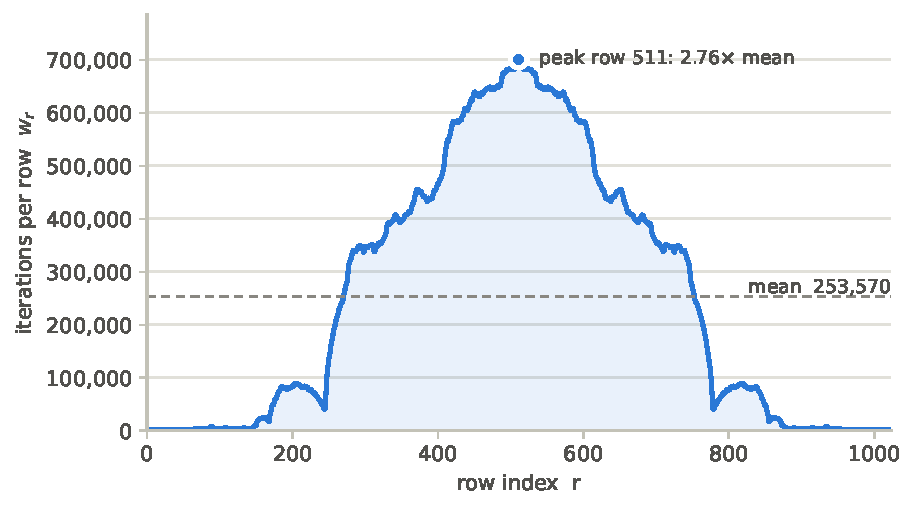
\includegraphics[width=0.85\textwidth]{Immagini/grafici/row_profile}
    \caption{Profilo di carico per riga $w_r$ della baseline seriale ($1024^2$,
    $N_{\max}=1000$, kernel \emph{bare}). La linea tratteggiata indica la media;
    il punto segna la riga di picco, che richiede $2{,}76$ volte le iterazioni
    medie.}
    \label{fig:serial-row-profile}
\end{figure}

\paragraph{Dalla baseline alle previsioni.}
Il profilo $\{w_r\}$ e la matrice degli escape time misurati in questa sezione
non si limitano a caratterizzare la baseline: bastano a prevedere il
comportamento delle versioni parallele prima che queste esistano. Le previsioni
sono tuttavia presentate insieme ai paradigmi cui si riferiscono, dove i
meccanismi che le giustificano sono già stati introdotti: i limiti di speedup
delle tre regole di assegnamento delle righe nella
sezione~\ref{sec:serial-pred-lambdaP}, il predittore della versione GPU nella
sezione~\ref{sec:cuda-previsioni}.
